\chapter{Mechanik}

\section{Kinematik}
Beschreibung von Bewegungen \\
einfachster Fall:
\begin{itemize}
	\item geradlinige Bahn (1D)
	\item gleichförmige Bewegung
\end{itemize}
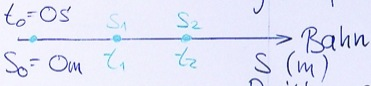
\includegraphics{Bild1}

\subsection{Weg-Zeit-Diagramm}
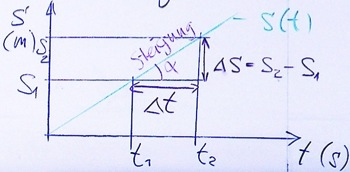
\includegraphics{Bild2}
\[ \tan \alpha = \frac{\Delta s}{\Delta t} \overset{!}{=} v \]
konst. Steigung von $s(t) \implies$ konst. $v$

\subsection{Geschwindigkeit}
\begin{def*}[ note = Geschwindigkeit , index = Geschwindigkeit ]
	\begin{gather*}
		v = \frac{\Delta s}{\Delta t} \\
		[v] = \frac{m}{s}
	\end{gather*}
\end{def*}

\subsection{Geschwindigkeits-Zeit Diagramm}
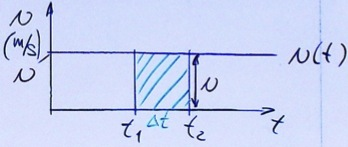
\includegraphics{Bild3}
\begin{gather*}
	v(t) = \frac{\Delta s}{\Delta t} \\
	\text{Fläche} = v \cdot \Delta t = \Delta s \text{ ! } = \text{ zurückgelegter Weg}
\end{gather*}

\subsection{Nicht-gleichförmige Bewegungen}
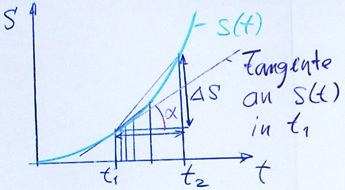
\includegraphics{Bild4}
Geschwindigkeit $v(t)$
\begin{gather*}
	\overline{v} = \frac{\Delta s}{\Delta t} = \text{ mittlere Geschwindigkeit zw. $t_1$ und $t_2$} \\
	v(t_1) = \lim_{t_1 \rightarrow t_2} \frac{\Delta s}{\Delta t} \underset{\text{\scriptsize{Math.}}}{=} s'(t) \\
	v(t) = s'(t) \\
\end{gather*}

\subsubsection{Schreibweise}
\begin{gather*}
	\Delta t \rightsquigarrow \dd t \\
	v(t) = s'(t) \eqqcolon \frac{\dd s}{\dd t}
\end{gather*}
1. Ableitung \\
$v(t)$: Momentangeschwindigkeit
\begin{bsp*}[ note = $v$ nimmt gleichmässig zu ]
	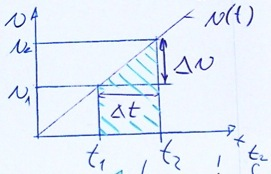
\includegraphics{Bild5}
	\[ \text{Fläche } \underset{\text{\scriptsize{Math.}}}{\overset{!}{=}} \int_{t_1}^{t_2} v(t) \dd t \]
\end{bsp*}
\todo{Undefined seq.}
Änderung der Geschwindigkeit mit der Zeit:
\begin{def*}[ note = Beschleunigung , index = Beschleunigung ]
	\begin{gather*}
		a = \frac{\Delta v}{\Delta t} \\
		[a] = \frac{m}{s^2}
	\end{gather*}
\end{def*}
Fall:
\begin{itemize}
	\item gleichförmige Beschleunigung: $a =$ konst.
	\item beliebige Funktion $a(t)$
\end{itemize}
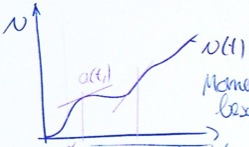
\includegraphics{Bild6}
analog:
\begin{gather*}
	a(t) = \frac{\dd v}{\dd t} \\
	a(t) = \frac{\dd}{\dd t} \left( \frac{\dd s}{\dd t} \right) = s''(t) \eqqcolon \frac{\dd^2 s}{\dd t^2}
\end{gather*}

\begin{rep*}[note = Kinematik (1D-Fall)]
	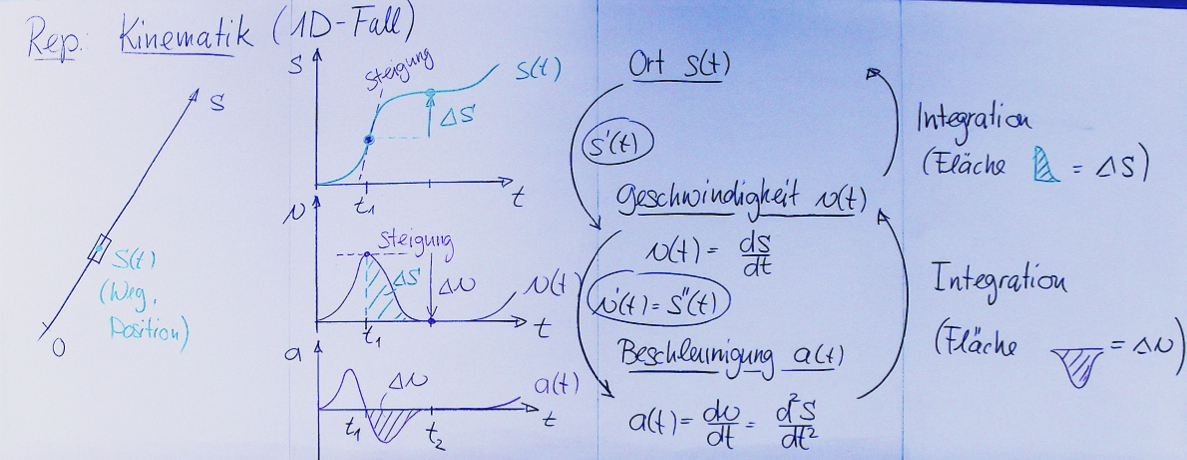
\includegraphics{Bild7}
\end{rep*}
\begin{bsp*}[note = Der freie Fall]
	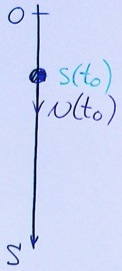
\includegraphics{Bild8} \\
	auf der Erdoberfläche
	\[ a(t) = a_{\text{Fall}} = g = 9.81 \frac{\text{m}}{{\text{s}}^2} \]
	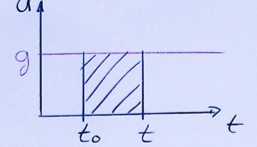
\includegraphics{Bild9}
	\[ \text{Fläche } = g( t - t_0 ) \]
	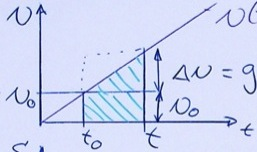
\includegraphics{Bild10}
	\begin{gather*}
		v(t) = v_0 + g( t - t_0 ) \\
		\Delta v = g( t - t_0 ) \
		\text{Fläche } = v_0 ( t - t_0 ) + \frac{1}{2} g( t - t_0 )^2 = \Delta S
	\end{gather*}
	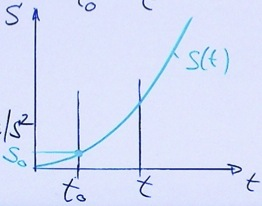
\includegraphics{Bild11}
	\[ s(t) = s_0 + v_0 ( t - t_0 ) + \frac{1}{2} g( t - t_0 ) \]
	
	einfachster Fall:
	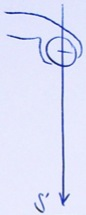
\includegraphics{Bild12}
	\begin{gather*}
		s(0) = 0 \\
		t_0 = 0 \\
		s_0 = 0 \\
		v_0 = 0 \\
		\implies s(t) = \frac{1}{2} gt^2
	\end{gather*}
\end{bsp*}

\subsection{Bewegungen in der Ebene}
\subsubsection{Ortsvektor \texorpdfstring{$\vec{r}(t)$}{r(t)}}
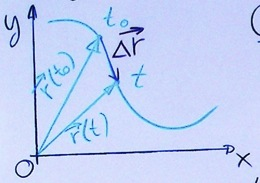
\includegraphics{Bild13}
\begin{itemize}[label = $\rightarrow$]
	\item Länge (Betrag)
	\item Richtung
\end{itemize}

Geschwindigkeit: $\frac{\text{Weg}}{\text{Zeit}}$
Weg: $\Delta \vec{r} = \vec{r}(t) - \vec{r}(t_0)$ \\
$\vec{v} = \frac{\Delta \vec{r}}{\Delta t}$ mittlere Geschwindigkeit \\
Momentangeschwindigkeit: $\vec{v}(t) = \lim_{\Delta t \rightarrow 0} \frac{\Delta \vec{r}}{\Delta t} \overset{\text{\scriptsize{Math.}}}{=} \frac{\dd \vec{r}}{\dd t}$ \\
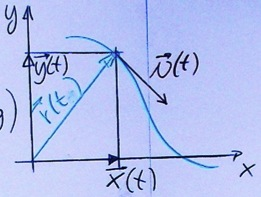
\includegraphics{Bild14}
\begin{gather*}
	\vec{r}(t) = \vec{x}(t) + \vec{y}(t) \\
	\implies \text{ Komponentenschreibweise} \\
	\vec{r}(t) = ( x(t) , y(t) ) \\
	\frac{\dd \vec{r}}{\dd t} = \left( \frac{\dd x}{\dd t} , \frac{\dd y}{\dd t} \right)
\end{gather*}
$v(t)$:
\begin{itemize}
	\item Betrag (Schnelligkeit)
	\item Richtung! (tangential zu Bahn)
\end{itemize}
\subsubsection{Schnelligkeit}
\[ \abs{\vec{v}(t)} = v(t) = \sqrt{{v_1}^2(t) + {v_2}^2(t)} \]
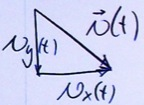
\includegraphics{Bild15}

\subsubsection{Momentanbeschleunigung}
\[ \vec{a}(t) = \frac{\dd \vec{v}}{\dd t} = \frac{\dd^2 \vec{s}}{\dd t^2} \]

\subsection{Wann ist eine Bewegung beschleunigt?}
Wenn $\vec{v}$ sich ändert!
\begin{itemize}[label = $\rightarrow$]
	\item Betrag
	\item Richtung!
\end{itemize}
\begin{bsp*}[note = Kreisbewegung mit konstante Umlaufgeschwindigkeit]
	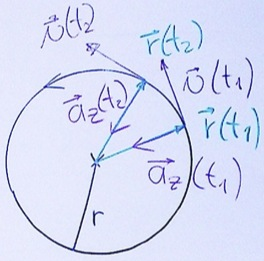
\includegraphics{Bild16}\\
	$\implies v =$ konst., $\vec{v}$ dreht $\implies$ Zentripetalbeschleunigung
	\[ a = \frac{v^2}{r} \]
\end{bsp*}
\begin{bsp*}[note = beliebige Kreisbewegung ($v \neq$ konst.)]
	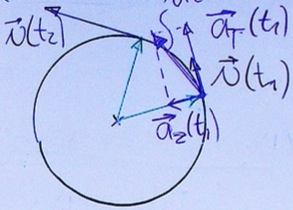
\includegraphics{Bild17} \\
	\[ \begin{matrix*}[l]
		a_Z(t) = \frac{v^2(t)}{r}		&\text{Zentripetalbeschleunigung} \\
		a_T(t) = \frac{\dd v}{\dd t}	&\text{Tangentialbeschleunigung}
	\end{matrix*} \]
\end{bsp*}

\subsection{Bewegungen im 3D-Raum}
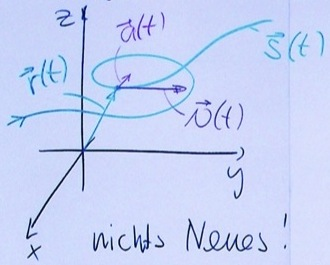
\includegraphics{Bild18} \\
nicht Neues!
\[ \vec{r}(t) = ( x(t) , y(t) , z(t) ) \]

\section{Dynamik}
$\implies$ Ursache der Bewegung
\subsection{Kraft/Masse}
\begin{def*}[ note = Kraft , index = Kraft ]
	\dots Wirkung!
\end{def*}
\begin{bsp*}
	\begin{itemize}
		\item Gewicht heben
		\item Deformation (Messung!)
		\item Bewegung
	\end{itemize}
\end{bsp*}
\begin{def*}[ note = Masse , index = Masse ]
	\enquote{Trägheit} (\enquote{\dots schwieriger in Bewegung zu setzen})
\end{def*}
Kraft: Vektor! \\
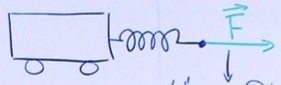
\includegraphics{Bild19} \\
Länge, Richtung, Angriffspunkt

\subsection{Die Newtonschen Prinzipien (1686)}
\begin{gather*}
	\underbrace{\vec{F}}_{\text{Ursache}} = \underbrace{m \cdot \vec{a}}_{\text{Wirkung}} \\
	[F] = \text{kg} \frac{\text{m}}{\text{s}^2} = \text{N} \quad ( \text{Newton} )
\end{gather*}
$\implies$ 2. Newtonsche Prinzip (Axiom) (Aktionsprinzip) \\
Anwendung: \\
\begin{itemize}
	\item Mann kennt Kraft $\implies$ Beschleunigung + Bahn berechnen
	\item Ich sehe Beschleunigung $\implies$ Was für Kräfte wirken
\end{itemize}
\subsubsection{1. Newtonsches Prinzip (Trägheitsprinzip)}
kräftefreie Körper ( $\vec{F} = \vec{0}$ , $\sum_i \vec{F_i} = \vec{0}$ )
\begin{itemize}[ label = $\rightarrow$ ]
	\item Körper in Ruhe (ist + bleibt)
	\item bewegt sich mit konst. Geschwindigkeit $\vec{v} =$ konst.
\end{itemize}
$\implies$ Bewegungszustände

\subsubsection{Newtonsches Prinzip (Reaktionsprinzip)}
(action = reactio) \\
Kräfte rühren immer von Wechselwirkungen (WW)
\begin{bsp*}[note = Feder]
	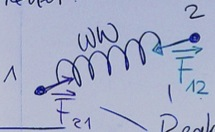
\includegraphics{Bild20}
	\[ \vec{F_{21}} = -\vec{F_{12}} \]
	Reaktionspartner $\rightarrow$ greifen immer an verschiedenen Körper an
\end{bsp*}
\begin{rep*}[ note = Dynamik ]
	Kraft: erzeugt Bewegung \\
	Masse: Trägheit \\
	Newtonsche Prinzipien \\
	\begin{enumerate}
		\item kräftefreier Körper: $\vec{v} =$ konst. (z.B. $\vec{v} = \vec{0}$)
		\item $\vec{F} = m \vec{a}$ Ursache \& Wirkung
		\item Kräfte rühren \textbf{immer} von WW her \\
			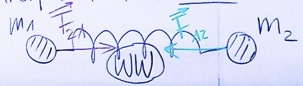
\includegraphics{Bild21} \\
			$\vec{F_{21}} = -\vec{F_12}$
	\end{enumerate}
\end{rep*}
\begin{bsp*}[ note = Hammer \& Nagel ]
	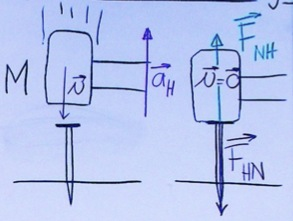
\includegraphics{Bild22}
	\begin{enumerate}[start = 2]
		\item $\vec{F_{NH}} = M \vec{a_H}$
		\item $\vec{F_HN} = -\vec{F_{NH}}$
	\end{enumerate}
\end{bsp*}

\subsection{Arten von Kräften}
\subsubsection{Gravitationskraft}
(Anziehung von Massen) \\
auf Erdoberfläche Gewichtskraft $\vec{G}$ \\
\begin{tabular}{ll}
	Betrag:			&$mg$ \\
	Richtung:			&zum Erdmittelpunkt \\
	Angriffspunkt:	&Schwerpunkt \\
	Reaktionspartner:	&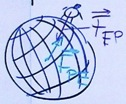
\includegraphics{Bild23}
\end{tabular}

\subsubsection{Elektromagnetische Kräfte}
(Anziehung / Abstossung von Ladungen)
\begin{itemize}[ label = $\rightarrow$ ]
	\item Coulombkraft (elektrische Kraft; verschiedene Erscheingungsformen)
	\item magnetische Kraft
	\item Lorentzkraft
\end{itemize}

\subsubsection{starke Kraft}
\begin{itemize}[ label = $\rightarrow$ ]
	\item Stabilität der Atomkeime
\end{itemize}

\subsubsection{schwache Kraft}
\begin{itemize}[ label = $\rightarrow$ ]
	\item Radioaktivität
\end{itemize}

\subsection{Coulombkraft und ihre Erscheinungsformen}
\begin{itemize}
	\item elastische Kräfte im festen Körpern (Kohäsion)
	\item Berührungskräfte - Die Normalkraft
		\begin{bsp*}[ note = Quader auf Tisch in Ruhe ]
			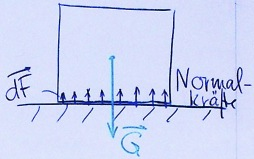
\includegraphics{Bild24}
			\begin{gather*}
				\sum \vec{F_a} = \vec{0} \\
				\implies \vec{G} + \sum \vec{\dd F} = \vec{0}
			\end{gather*}
		\end{bsp*}
\end{itemize}

\subsubsection{Coulombgesetz}
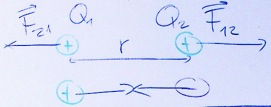
\includegraphics{Bild25}
\[ F_{21} = F_{12} = \frac{1}{4 \pi \epsilon_0} \frac{Q_1 Q_2}{r^2} \]
elektirsche Feldkonstante $\epsilon_0 = 8.85 \cdot 10^{-12} \frac{\text{As}}{\text{Vm}}$

\subsubsection{Kraftgesetz zwischen zwei Atomen}
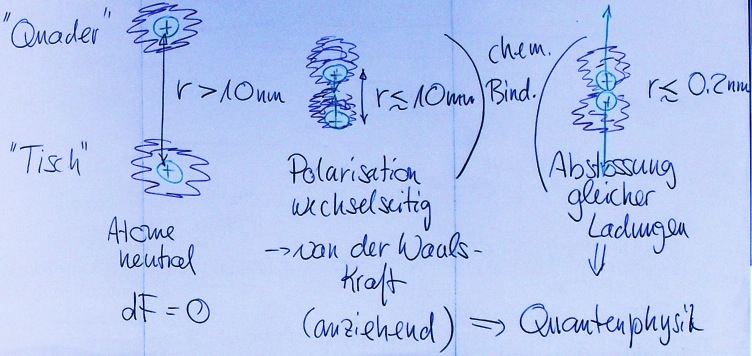
\includegraphics{Bild26}

\subsubsection{Kraftkurve}
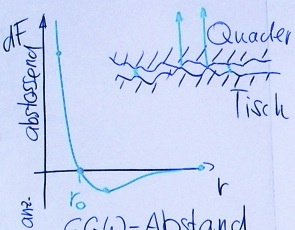
\includegraphics{Bild27} \\
GGW-Abstand (chemische Bindung)

\subsection{Reibungskräfte}
(parallel zur Berührungsfläche)

\subsubsection{Haftreibung}
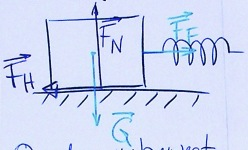
\includegraphics{Bild28} \\
Quader unbewegt \\
\[ \vec{F_H} = -\vec{F_F} \]

maximale Haftreibung:
\[ F_H \leq \underbrace{\mu_H}_{\text{Haftreibungszahl}} F_N \]

\subsection{Gleitreibung \texorpdfstring{$\vec{F_R}$}{F_R}}
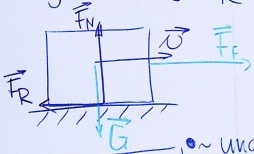
\includegraphics{Bild29}
\begin{itemize}
	\item Richtung: versucht immer Relativbewegung zu bremsen.
	\item unabhängig von $v$
\end{itemize}
\[ F_R = \mu_G \cdot F_N \]

\subsection{Kraftstösse}
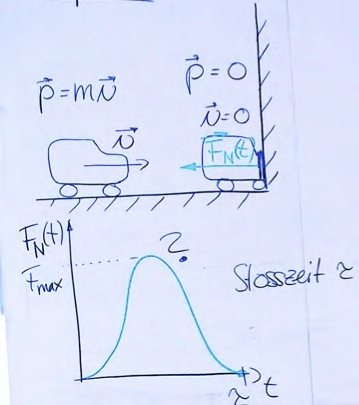
\includegraphics{Bild30}
\begin{rep*}
	Atomic Force Microscope (AFM) \\
	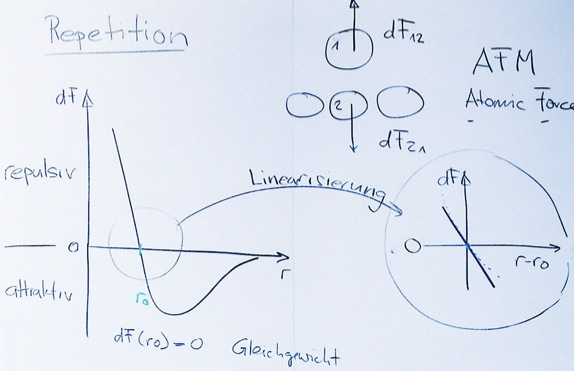
\includegraphics{Bild31}
	\[ \dd F =  -D ( r - r_0 ) = -\underbrace{D}_{\text{Federkonstante}} \cdot \underbrace{x}_{\text{Auslenkung}} \]
	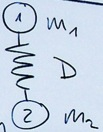
\includegraphics{Bild32}
	\[ D( \ce{O2} ) \approx 1200 \frac{\text{N}}{\text{m}} \]
\end{rep*}
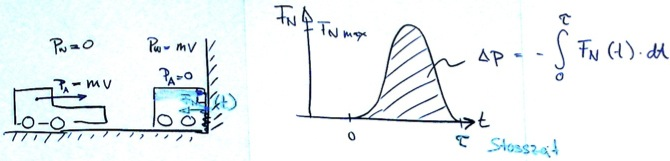
\includegraphics{Bild33}
\[ \Delta p = -\int_0^\tau F_n(t) \cdot \dd t \]
$\tau$ Stosszeit \\
kleine Kräfte $F_N$:
\begin{itemize}
	\item wenn $\tau$ gross
	\item wenn $\Delta p$ klein
\end{itemize}

\subsubsection{Experiment}
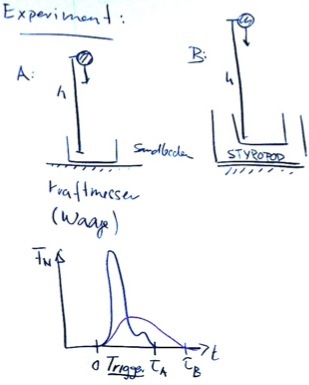
\includegraphics{Bild34}

\subsubsection{Vereinfachung}
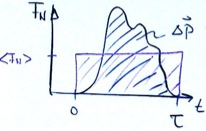
\includegraphics{Bild35}
\[ \Delta \vec{p} = m \vec{v} = - \scal{\vec{F_N}} \tau = - \int_0^\tau F_N(t) \dd t \]

\subsection{Das Drehmoment}
\begin{def*}[ note = Drehmoment , index = Drehmoment ]
	\[ \vec{M_0} = \vec{r} \times \vec{F} \]
\end{def*}
(Hebelgesetz) \\
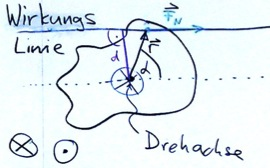
\includegraphics{Bild36}
\[ M_0 = r \cdot F_N \cdot \sin \alpha = \dd F_N \]
Rechte-Hand-Regel: \\
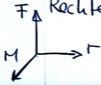
\includegraphics{Bild37}

\subsection{Gleichgewicht starrer Körper}
keine Bewegung:
\begin{gather*}
	\sum \vec{F_i} = 0 \quad \text{Translation} \\
	\sum \vec{M_i} = 0 \quad \text{Rotation}
\end{gather*}

\subsection{Der Schwerpunkt SP}
\begin{def*}[ note = Schwerpunkt , index = Schwerpunkt ]
	\[ \vec{r_s} = \frac{\sum \overbrace{m_i}^{\text{Massenelement}} r_i}{\sum m_i} \]
\end{def*}
gewichtetes  Mittel aller Orte der Körpermassen und ist der Angriffspunkt der Gewichtskraft \\
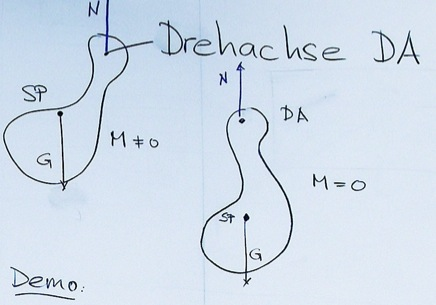
\includegraphics{Bild38}

\subsubsection{Denkexperiment Spazierstock}
Schwerpunkt des \\
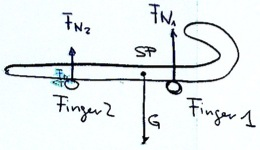
\includegraphics{Bild39} \\
wenn $F_{R_1} > F_{R_2}$ bewegt sich Finger 2.

\section{Festigkeitslehre (Elastizitätslehre)}
Reale Körper sind deformierbar (reversibel und/oder irreversibel). Festigkeit hängt vom Material und Form ab. \\
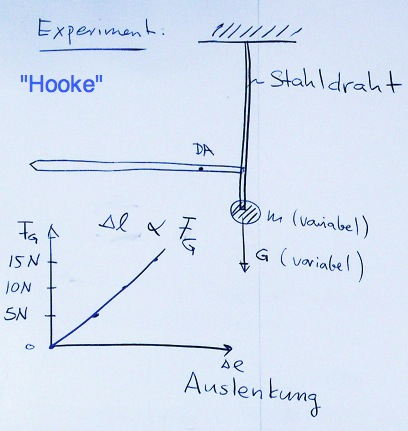
\includegraphics{Bild40}

\subsection{Materialverhalten}
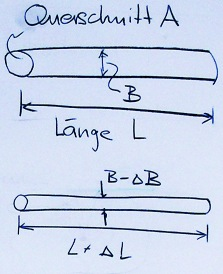
\includegraphics{Bild41} \\
\begin{def*}[ note = Dehnung , index = Dehnung ]
	\begin{gather*}
		\epsilon = \frac{\Delta L}{L} \\
		[ \epsilon ] = 1
	\end{gather*}
\end{def*}
\begin{def*}[ note = Querkontraktion , index = Querkontraktion ]
	\[ \beta = \frac{\Delta B}{B} \]
\end{def*}
\begin{def*}[ note = Normalspannung , index = Normalspannung ]
	\begin{gather*}
		\sigma = \frac{F_N}{A} \\
		[ \sigma ] = \text{Pa}
	\end{gather*}
	Zugspannung $\sigma > 0$ \\
	Druckspannung $\sigma < 0$
\end{def*}

\subsubsection{Das Spannungs-Dehnungs Diagramm}
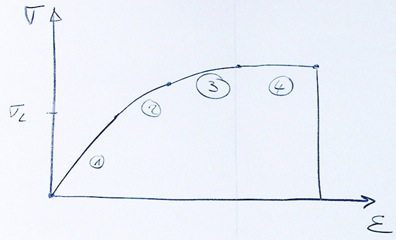
\includegraphics{Bild42} \\
\begin{enumerate}
	\item linearer Bereich $\sigma = E \epsilon$\footnote{$E$ Elastizitätsmodul, z.B. Stahl 200 GPa , Nanotubes 1TPa}
	\item nichtlinearer Bereich
	\item plastischer Bereich
	\item Fliessen
	\item Bruch
\end{enumerate}

\begin{rep*}
	\begin{itemize}
		\item Kraftstoss $\vec{F} \cdot \Delta t = \Delta \vec{p}$
		\item Derhmoment $\vec{M_o} = \vec{r} \times \vec{F}$ \\
			(Folien) \\
			gerichtete Grösse mit Drehsinn \\
			rechte Hand Regel \\
			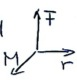
\includegraphics{Bild43}
		\item Schwerpunkt $\vec{r_{SP}} = \frac{\sum m_i \vec{r_i}}{\sum m_i}$
	\end{itemize}
	Festigkeitslehre \\
	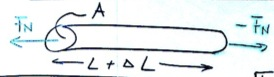
\includegraphics{Bild44} \\
	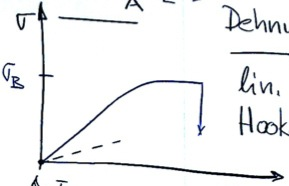
\includegraphics{Bild45}
	\begin{bsp*}
		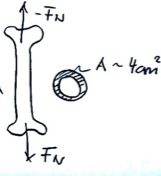
\includegraphics{Bild46}
		\[
			\sigma_{B \text{ Knochen}} = 85 \text{MPa} \\
			\implies F_{N \text{ max}} = \sigma_B \cdot A = 34 \text{kN}
		\]
	\end{bsp*}
	Spannungs-Dehnungsdiagramm \\
	lin. Bereich Hooke'sches Gesetz:
	\[
		\sigma = \underbrace{E}_{\text{Elastizitätsmodul}} \cdot \epsilon \\
		\epsilon = \frac{\Delta L}{L} \quad []
	\]
\end{rep*}

\subsection{Scherung}
Demo: Schaumgummiquader \\
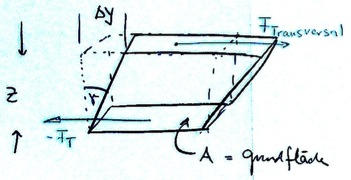
\includegraphics{Bild47} \\
Scherwinkel
\[ \gamma = \frac{\Delta y}{z} \]
\begin{def*}[ note = Schubspannung , index = Schubspannung ]
	\[
		\tau = \frac{F_T}{A} \\
		[ \tau ] = \text{Pa}
	\]
	für den linearen Bereich (Hooke) gilt:
	\[ \tau = \underbrace{G}_{\text{Schubmodul } [ \text{Pa} ]} \cdot \gamma \]
\end{def*}

\subsection{Spannungszustand}
Dehnung, Staucherung \\
Scherung, Biegung \\
Torsion \\
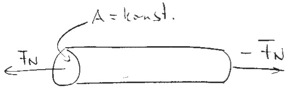
\includegraphics{Bild48} \\
Spannungsfelder
\[
	\sigma( x , y , z ) = \sigma(\vec{r}) = \frac{F_N}{A} = \text{ konst.} \\
	\tau(\vec{r}) = 0 \quad (\text{keine Scherung})
\]
Die Spannung in einem Körper lässt sich für jeden Punkt bestimmen.

\subsection{Die Biegebelastung eines Balkens}
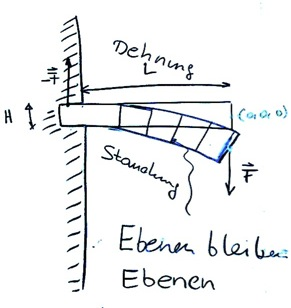
\includegraphics{Bild49} \\
Querschnitt $A = H \cdot B$ \\
Biegung:
\begin{itemize}
	\item $\sigma$ Normalspannung
	\item $\tau$ Schubspannungen
\end{itemize}
Problem: Bestimmung von $\sigma(\vec{r}) ; \tau(\vec{r})$ unter Berücksichtigung des Gleichgewichts

\subsubsection{Wahl des Koordinatensystems}
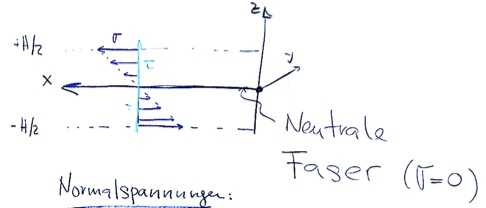
\includegraphics{Bild50} \\
Normalspannungen:
\[ \sigma( x , y , z ) = \alpha(x) \cdot z \]
prop. zur Dehnung. \\
Annahme: Gewichts des Balken $\ll F$ \\
Kräfte Gleichgewicht: \\
$z$-Komonente
\[ - F + A \cdot \tau(x) = 0 \implies \tau(x) = \frac{F}{A} = \text{ konst.} \]
$x$-Komponente:
\[
	\int_A \sigma( x , y , z ) \dd A = 0 \\
	\implies \int_{-\frac{H}{2}}^{+\frac{H}{2}} \alpha(x) \cdot z \cdot B \cdot \dd z = 0 \\
	\implies \alpha(x) \cdot B \underbrace{\int_{-\frac{H}{2}}^{+\frac{H}{2}} z \cdot \dd z}_{\text{muss $0$ sein}} = 0 \\
	\implies \text{ neutrale Faser liegt in der Mitte}
\]

\subsection{Drehmomentgleichgewicht}
\[
	\abs{M_\curvearrowright} = F \cdot x \\
	\abs{M_\curvearrowleft} = \int_A z \cdot \sigma( x , y , z ) \cdot \dd A \\
	\text{Gleichgewicht: } \abs{M_\curvearrowright} = \abs{M_\curvearrowleft} \\
	F \cdot x = \int_A z \cdot \alpha(x) \cdot z \cdot \dd A = \alpha(x) \cdot \underbrace{\overbrace{\int_A z^2 \dd A}^{\text{geometrischer Faktor}}}_{\text{Flächenträgheitsmoment } I_z} \\
	\implies \alpha( x , z ) = \alpha( x ) \cdot z = \frac{x \cdot z}{I_z} \cdot F
\]
Diskussion:
\begin{itemize}
	\item Neutrale Faser leigt bei $z=0$
	\item wo bricht der Balken bei $( L , y , \frac{H}{2} )$
	\item $I_z = \frac{1}{12} BH^3$ \\
		\includegraphics{Bild51}
\end{itemize}



























